\documentclass[12pt, oneside]{article} 
% \documentclass{article} 
\usepackage{amsmath, amsthm, amssymb, calrsfs, wasysym, verbatim, bbm, 
                color, graphics, geometry}
\usepackage{fancyvrb} % for "\Verb" macro
\usepackage[toc,page]{appendix}
\usepackage[pdftex]{graphicx}
\usepackage{float}
\usepackage{hyperref}
\usepackage{mathtools}


\usepackage{subcaption}

\hypersetup{
    colorlinks=true,
    linkcolor=blue,
    filecolor=magenta,      
    urlcolor=cyan,
}
 
\urlstyle{same}

\geometry{tmargin=1.25in, bmargin=1.25in, lmargin=1.00in, rmargin = 1.00in}  

\newcommand{\R}{\mathbb{R}}
\newcommand{\C}{\mathbb{C}}
\newcommand{\Z}{\mathbb{Z}}
\newcommand{\N}{\mathbb{N}}
\newcommand{\Q}{\mathbb{Q}}
\newcommand{\Cdot}{\boldsymbol{\cdot}}

\usepackage{listings}
\usepackage{color} %red, green, blue, yellow, cyan, magenta, black, white
\definecolor{mygreen}{RGB}{28,172,0} % color values Red, Green, Blue
\definecolor{mylilas}{RGB}{170,55,241}

\title{CIS580 PSet 3}
\author{Sheil Sarda}
\date{02.24.2021}

\begin{document}
\lstset{language=Matlab,%
    %basicstyle=\color{red},
    breaklines=true,%
    morekeywords={matlab2tikz},
    keywordstyle=\color{blue},%
    morekeywords=[2]{1}, keywordstyle=[2]{\color{black}},
    identifierstyle=\color{black},%
    stringstyle=\color{mylilas},
    commentstyle=\color{mygreen},%
    showstringspaces=false,%without this there will be a 
    % symbol in the places where there is a space
    numbers=left,%
    numberstyle={\tiny \color{black}},% size of the numbers
    numbersep=9pt, % this defines how far the numbers are from the text
    emph=[1]{for,end,break},emphstyle=[1]\color{red}, %some words to emphasise
    %emph=[2]{word1,word2}, emphstyle=[2]{style},    
}

\begin{titlepage}
    \begin{flushleft}
        \vspace*{1cm}
        \Huge
        \textbf{CIS580 Problem Set 7\\ }
        \vspace*{0.5cm}
        \normalsize
        Sheil Sarda \verb|<sheils@seas.upenn.edu>| \\
        CIS580 Spring 2021
        \tableofcontents
    \end{flushleft}
\end{titlepage}

\section{Scale Invariant Detection}

\subsection{Laplacian of Gaussian}

\begin{figure}[H]
    \centering
    \begin{subfigure}[b]{1\textwidth}
        \centering
        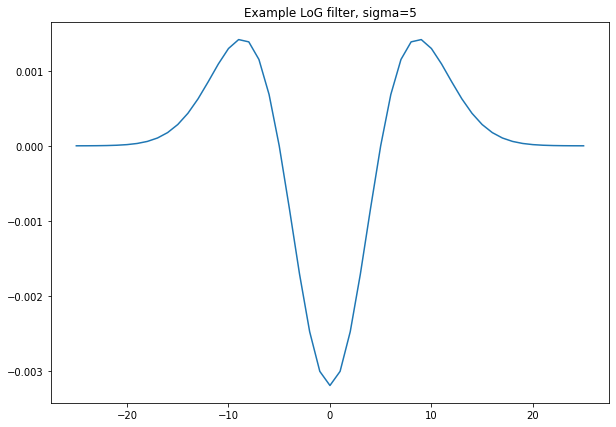
\includegraphics[width=\textwidth]{imgs/q1.1_plot.png}
    \end{subfigure}
    \caption{}
\end{figure}
\subsection{Approximating a LoG by a DoG}

\subsubsection{Difference of Gaussians}
\begin{figure}[H]
    \centering
    \begin{subfigure}[b]{0.8\textwidth}
        \centering
        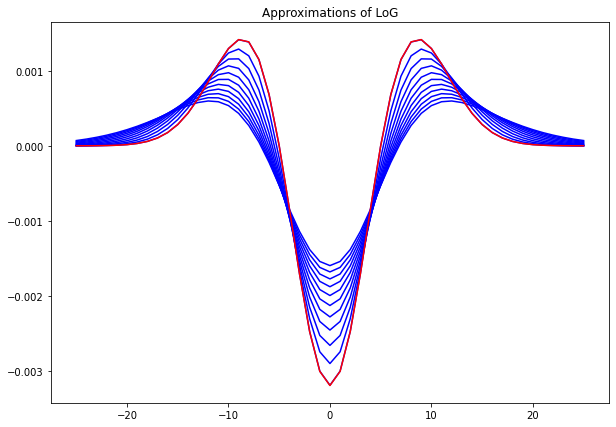
\includegraphics[width=\textwidth]{imgs/q1.2_plot1.png}
    \end{subfigure}
    \caption{}
\end{figure}
The plots obtained indicate that as $k$ increases from $1 \to 2$, the Difference of Gaussians approximation is scaled down in magnitude.	
\begin{figure}[H]
    \centering
    \begin{subfigure}[b]{0.4\textwidth}
        \centering
        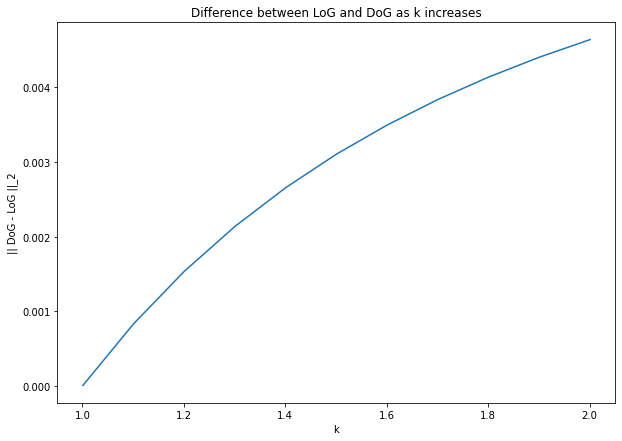
\includegraphics[width=\textwidth]{imgs/q1.2_plot2.png}
    \end{subfigure}
    \caption{}
\end{figure}
\subsubsection{DoG gets closer to LoG as $k \to 1$}
We exepect this to happen because in the provided expression, as $k \to 1$, the LoG will approach the DoG.
$$ \text{LoG}_\sigma = \frac{1}{(k - 1) \sigma^2}\text{DoG}_\sigma$$

\subsubsection{Dropping the normalizing factor}

We intentionally forget the normalizing factor and just use the difference of Gaussians because the product of a scalar and a Normal distribution will simply apply the constant as a scaling factor to both terms in the DoG expression.


\subsection{Detecting sunflowers}

\subsubsection{Sunflower detection}
\begin{figure}[H]
    \centering
    \begin{subfigure}[b]{1\textwidth}
        \centering
        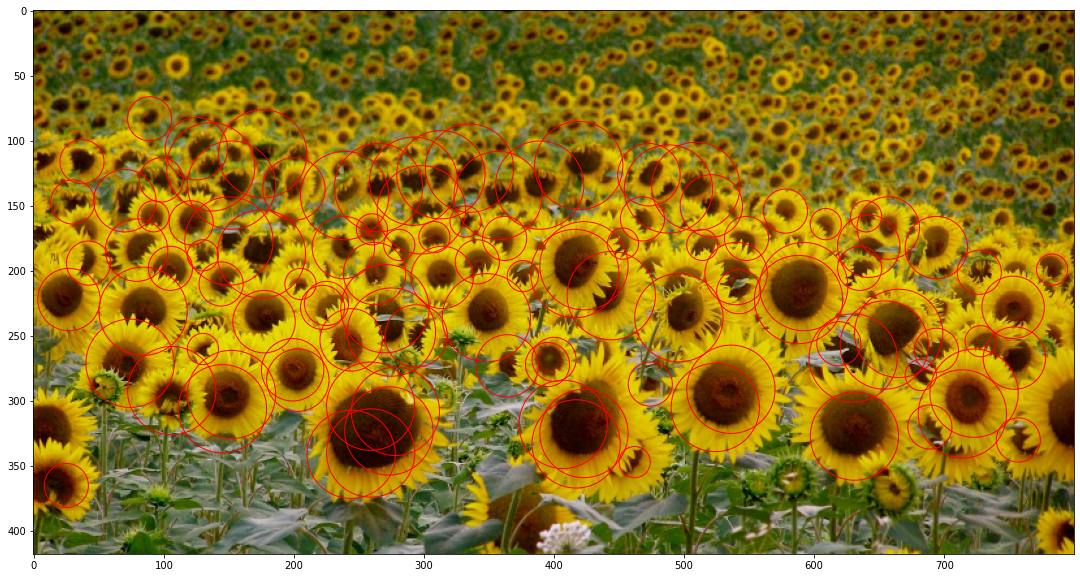
\includegraphics[width=\textwidth]{imgs/q1.3_plot1.png}
    \end{subfigure}
    \caption{}
\end{figure}

\subsubsection{Blob detection on custom image}
\begin{figure}[H]
    \centering
    \begin{subfigure}[b]{1\textwidth}
        \centering
        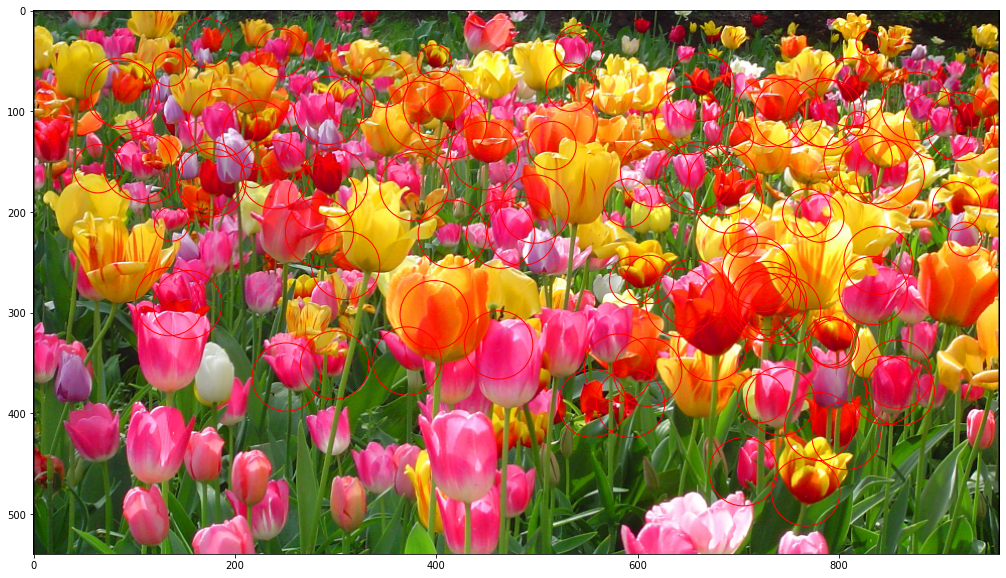
\includegraphics[width=\textwidth]{imgs/q1.3_plot2.png}
    \end{subfigure}
    \caption{}
\end{figure}

\section{Finding Waldo with Gabor Filters}

\subsection{Gabor Filter in 2D}
\begin{figure}[H]
    \centering
    \begin{subfigure}[b]{0.25\textwidth}
        \centering
        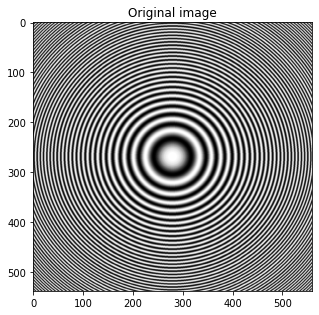
\includegraphics[width=\textwidth]{imgs/q2.1_plot1.png}
    \end{subfigure}
    \caption{Original Image}
\end{figure}

\begin{figure}[H]
    \centering
    \begin{subfigure}[b]{1\textwidth}
        \centering
        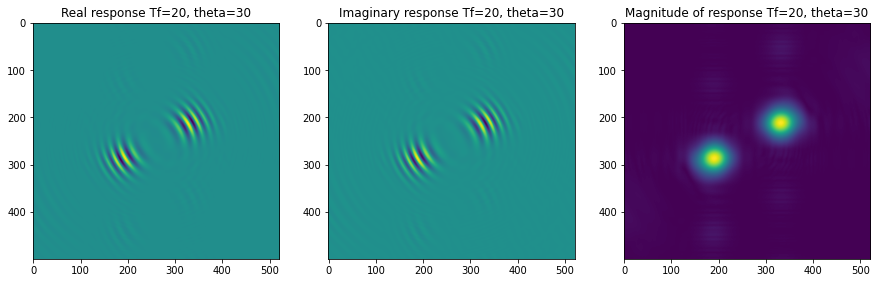
\includegraphics[width=\textwidth]{imgs/q2.1_plot2.png}
    \end{subfigure}
    \hfill
    \begin{subfigure}[b]{1\textwidth}
        \centering
        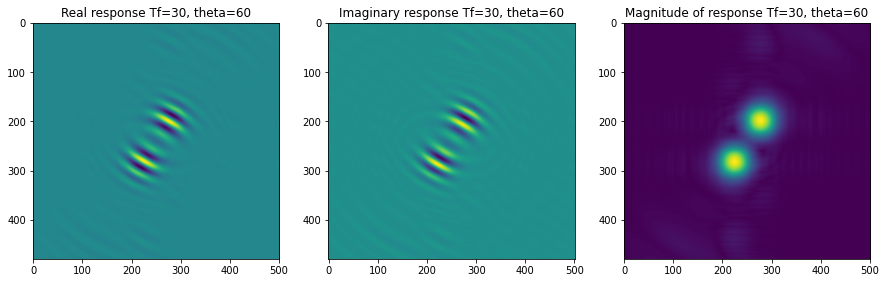
\includegraphics[width=\textwidth]{imgs/q2.1_plot3.png}
    \end{subfigure}
    \hfill
    \begin{subfigure}[b]{1\textwidth}
        \centering
        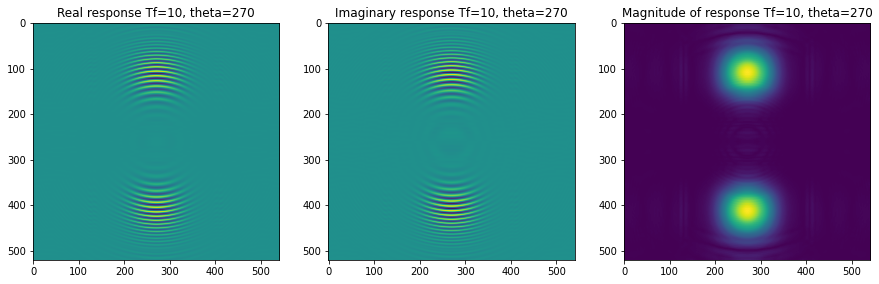
\includegraphics[width=\textwidth]{imgs/q2.1_plot4.png}
        \caption{$\sigma = 0.1$}
    \end{subfigure}
       \caption{Gabor 2D Plot with different parameters}
       \label{fig:three graphs}
\end{figure}

As the spatial period increases, the dots move away from the center. The angle we are using as offset determines the orientation of the image. We also notice that the magnitude of the response is inversely proportional to the distance from the center.

\subsection{Finding Waldo}

\subsubsection{Creation of im\_red}
The image is created by supressing the green and blue color channels from the RGB image. This helps convert the image to a grayscale image. The choice of suppressing the greens and blues by subtracting their average intensity might be impacted by the fact that we wish to maintain the whitespace in the image, which is represented by $\text{RGB}(255, 255, 255)$. Hence, if we eliminate the greens and blues, we will lose the white.

\begin{verbatim}
im_red = image[:,:,0] - 0.5*(image[:,:,1] + image[:,:,2]);
im_red[im_red < np.mean(im_red[:])] = np.mean(im_red[:]);
im_red = im_red - np.mean(im_red[:]);
\end{verbatim}

\subsubsection{Finding Waldo}

\begin{figure}[H]
    \centering
    \begin{subfigure}[b]{1\textwidth}
        \centering
        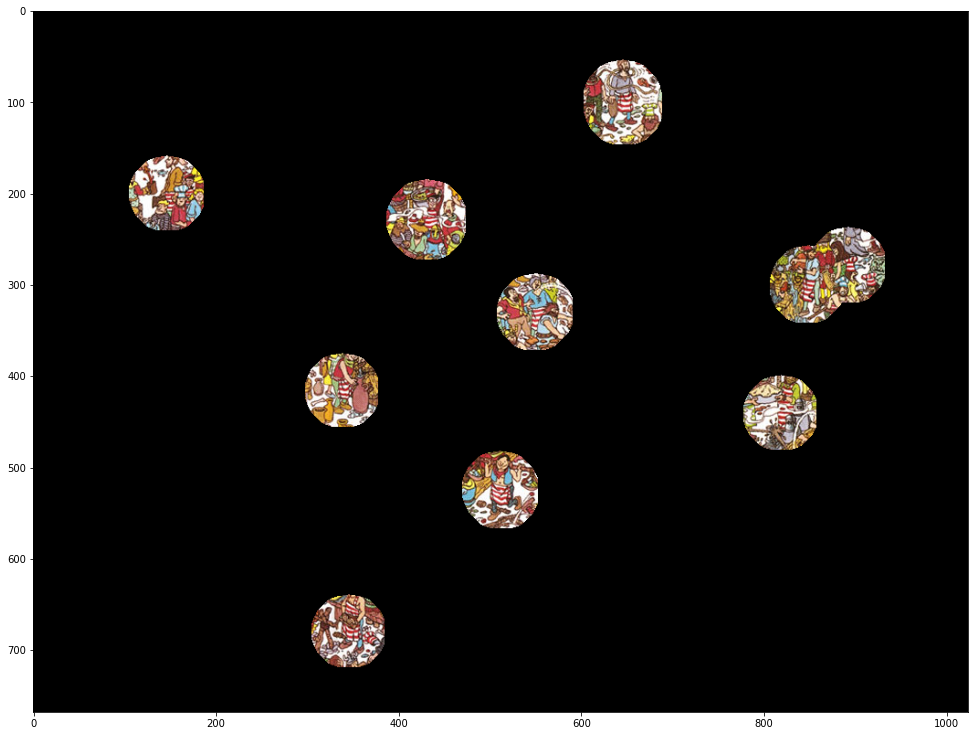
\includegraphics[width=\textwidth]{imgs/q2.2_plot.png}
    \end{subfigure}
    \caption{Masked Image with Waldo}
\end{figure}

Using the above masked image, we can find Waldo!

\begin{figure}[H]
    \centering
    \begin{subfigure}[b]{1\textwidth}
        \centering
        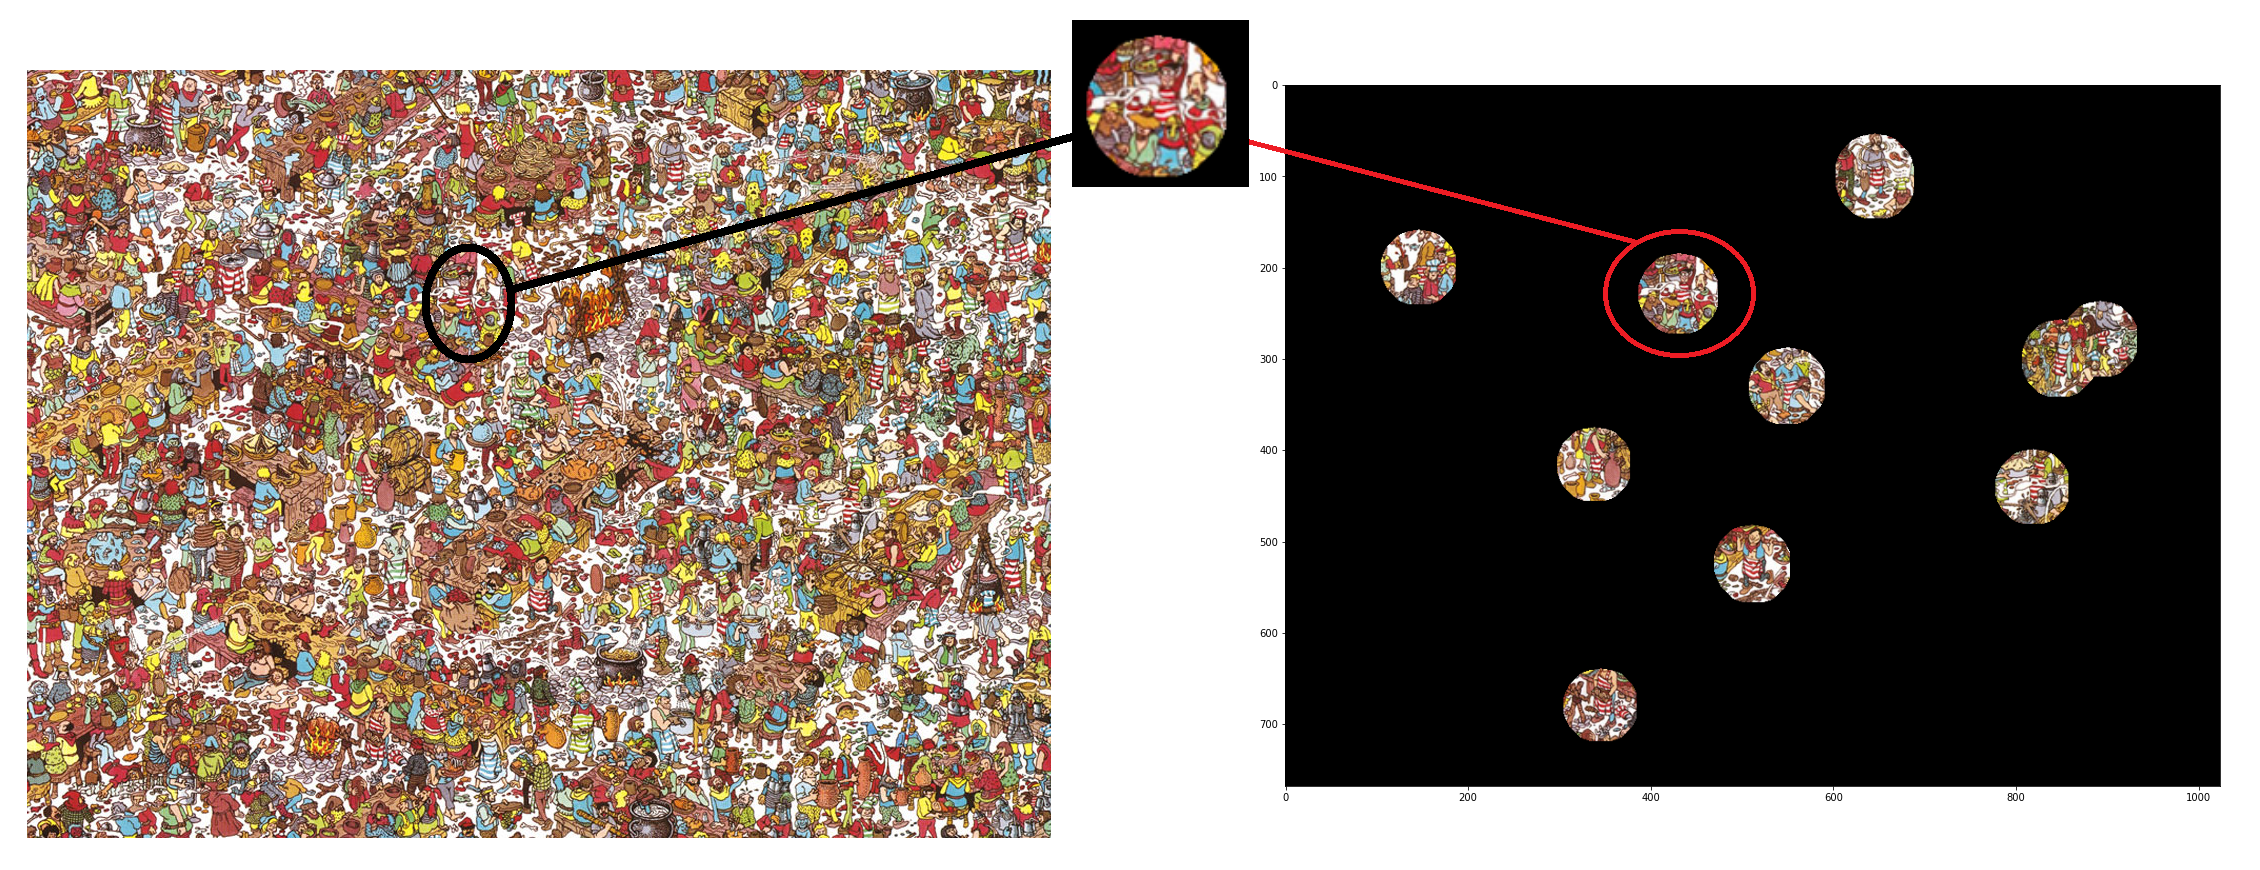
\includegraphics[width=\textwidth]{imgs/waldo_found.png}
    \end{subfigure}
\end{figure}

\end{document}
